% --- Chapter 3: Implementation ---
\chapter{Реалізація системи}
\label{ch:implementation}

\section{Огляд процесу розробки}
\label{sec:dev_process}
% TODO: Describe development methodology (e.g., Agile, Waterfall), tools used (Git, VS Code, Docker), and workflow.
Розробка веб-платформи для комунікації та обміну знаннями в спільноті бджолярів \textit{Beekeepers Community Platform} велася з використанням гнучких підходів, що дозволяли ітеративно додавати функціонал та вносити корективи. Основними інструментами розробки були Visual Studio Code як інтегроване середовище розробки, Git для системи контролю версій (з використанням GitHub для хостингу репозиторію), Docker та Docker Compose для контейнеризації та управління середовищем розробки та розгортання. Робочий процес включав регулярні коміти, розробку у функціональних гілках (за потреби) та тестування ключових функцій на локальному середовищі перед розгортанням.

\section{Організація коду}
\label{sec:code_organization}
Структура коду проекту організована для забезпечення модульності, легкості підтримки та масштабування.

\subsection{Структура проекту фронтенду}
Клієнтська частина (директорія \texttt{client/}) розроблена на React з використанням Vite як інструменту для збірки. Основні директорії в \texttt{src/}:
\begin{itemize}
    \item \texttt{components/}: Містить UI компоненти, розділені за функціональними ознаками (наприклад, \texttt{forum/}, \texttt{map/}, загальні компоненти).
    \item \texttt{pages/}: Компоненти, що відповідають за окремі сторінки застосунку (наприклад, \texttt{Home.tsx}, \texttt{Forums.tsx}, \texttt{MapPage.tsx}).
    \item \texttt{services/} (або \texttt{store/api/}): API-зрізи (slices) для RTK Query, що описують взаємодію з бекенд API (наприклад, \texttt{authApi.ts}, \texttt{forumApi.ts}, \texttt{mapApi.ts}).
    \item \texttt{store/}: Конфігурація Redux store (\texttt{store.ts}).
    \item \texttt{context/}: React Context API для управління глобальним станом, таким як автентифікація (\texttt{AuthContext.tsx}).
    \item \texttt{hooks/}: Спеціалізовані React хуки.
    \item \texttt{types/}: Загальні TypeScript типи та інтерфейси.
    \item \texttt{locales/}: Файли перекладів для інтернаціоналізації (\texttt{en/translation.json}, \texttt{uk/translation.json}).
    \item \texttt{utils/}: Допоміжні функції та утиліти.
    \item \texttt{App.tsx}: Головний компонент застосунку, що налаштовує маршрутизацію.
    \item \texttt{index.tsx} (або \texttt{main.tsx}): Вхідна точка застосунку.
\end{itemize}

\subsection{Структура проекту бекенду}
Серверна частина (директорія \texttt{server/}) розроблена на NestJS. Проект структурований за модульним принципом:
\begin{itemize}
    \item \texttt{src/}: Містить основний код застосунку.
    \item \texttt{src/MODULE\_NAME/}: Кожен функціональний блок (наприклад, \texttt{auth/}, \texttt{users/}, \texttt{forum/}, \texttt{hives/}, \texttt{fields/}, \texttt{health/}, \texttt{email/}) виділений в окремий модуль NestJS.
    \item Кожен модуль зазвичай містить:
        \begin{itemize}
            \item \texttt{*.module.ts}: Файл визначення модуля.
            \item \texttt{*.controller.ts}: Контролер, що обробляє запити за протоколом передачі гіпертексту (Hypertext Transfer Protocol, HTTP).
            \item \texttt{*.service.ts}: Сервіс, що інкапсулює бізнес-логіку.
            \item \texttt{schemas/}: Mongoose схеми для визначення структури даних MongoDB.
            \item \texttt{dto/}: Об'єкти передачі даних (Data Transfer Objects, DTOs) для валідації вхідних даних.
            \item \texttt{guards/}, \texttt{strategies/}, \texttt{decorators/}, \texttt{types/} (для специфічних типів модуля, наприклад, в \texttt{auth/}).
        \end{itemize}
    \item \texttt{src/main.ts}: Вхідна точка серверного застосунку, ініціалізація NestJS та Fastify.
    \item \texttt{src/app.module.ts}: Кореневий модуль застосунку.
\end{itemize}

\subsection{Проектування API}
Прикладний програмний інтерфейс (Application Programming Interface, API) спроектовано за принципами RESTful (Representational State Transfer). Всі кінцеві точки (ендпоінти) мають префікс \texttt{/api/v1/}, що забезпечує версіонування. Для валідації даних, що надходять від клієнта, використовуються об'єкти передачі даних (DTO) з декораторами \texttt{class-validator}. Документація API автоматично генерується за допомогою Swagger (OpenAPI) і доступна на ендпоінті \texttt{/docs} (у середовищі розробки), що спрощує тестування та інтеграцію.

\section{Опис ключових компонентів та модулів}
\label{sec:key_components}

\subsection{Автентифікація та авторизація}
Система автентифікації реалізована з використанням Passport.js. Підтримуються:
\begin{itemize}
    \item \textbf{Локальна стратегія:} Автентифікація за логіном (email) та паролем. Паролі зберігаються у хешованому вигляді (з використанням \texttt{crypto.pbkdf2Sync}).
    \item \textbf{JWT (JSON Web Tokens):} Використовуються для авторизації користувачів після успішного входу. Генеруються access та refresh токени.
    \item \textbf{Верифікація Email:} При реєстрації користувачу надсилається лист з унікальним токеном для підтвердження електронної пошти. Доступ до функціоналу обмежений до верифікації. Термін дії токена -- 1 година.
    \item \textbf{Повторне надсилання листа верифікації:} Реалізовано можливість для користувача запросити повторне надсилання листа для верифікації email, якщо попередній токен сплив або лист не було отримано. Цей функціонал включає новий ендпоінт API (\texttt{/auth/resend-verification-email}) та відповідний інтерфейс на сторінці верифікації (\texttt{VerifyEmailPage.tsx}).
    \item \textbf{Google OAuth 2.0:} Реалізовано можливість входу та реєстрації через обліковий запис Google. При натисканні кнопки "Увійти через Google" на сторінці входу (див. рисунок \ref{fig:login_page}), користувач перенаправляється на сторінку автентифікації Google. Після надання згоди, Google перенаправляє користувача назад до застосунку з авторизаційним кодом. Серверна частина обмінює цей код на токени доступу та інформацію про профіль користувача Google (email, ім\'я, фото). Бекенд-сервіс (\texttt{AuthService}, метод \texttt{findOrCreateGoogleUser}) перевіряє, чи існує користувач з таким email. Якщо так, користувач автентизується. Якщо ні, створюється новий обліковий запис, email автоматично позначається як верифікований, а для внутрішніх потреб генерується випадковий пароль (оскільки прямий вхід за паролем для таких акаунтів не передбачений). Після цього для користувача генеруються стандартні JWT (access та refresh токени) для подальшої роботи з платформою. Такий підхід спрощує процес реєстрації та входу для користувачів, підвищуючи зручність використання платформи.
    \item \textbf{Захист маршрутів (Guards):} \texttt{JwtAuthGuard} використовується для захисту ендпоінтів, що вимагають автентифікації. \texttt{LocalAuthGuard} використовується для обробки локального входу.
\end{itemize}

Для нових користувачів передбачено процес реєстрації, інтерфейс якого показаний на рисунку \ref{fig:registration_form}. Користувачу необхідно надати свою електронну адресу, обрати ім\'я користувача (username) та створити пароль. Після відправки форми, серверна частина виконує валідацію наданих даних. У випадку успішної валідації, створюється новий обліковий запис, пароль зберігається у хешованому вигляді, а для підтвердження електронної пошти генерується унікальний токен верифікації, який надсилається користувачу на вказану адресу. Цей крок є обов\\'язковим перед тим, як користувач зможе повноцінно увійти до системи та отримати доступ до її функціоналу.

\begin{figure}[htbp]
    \centering
    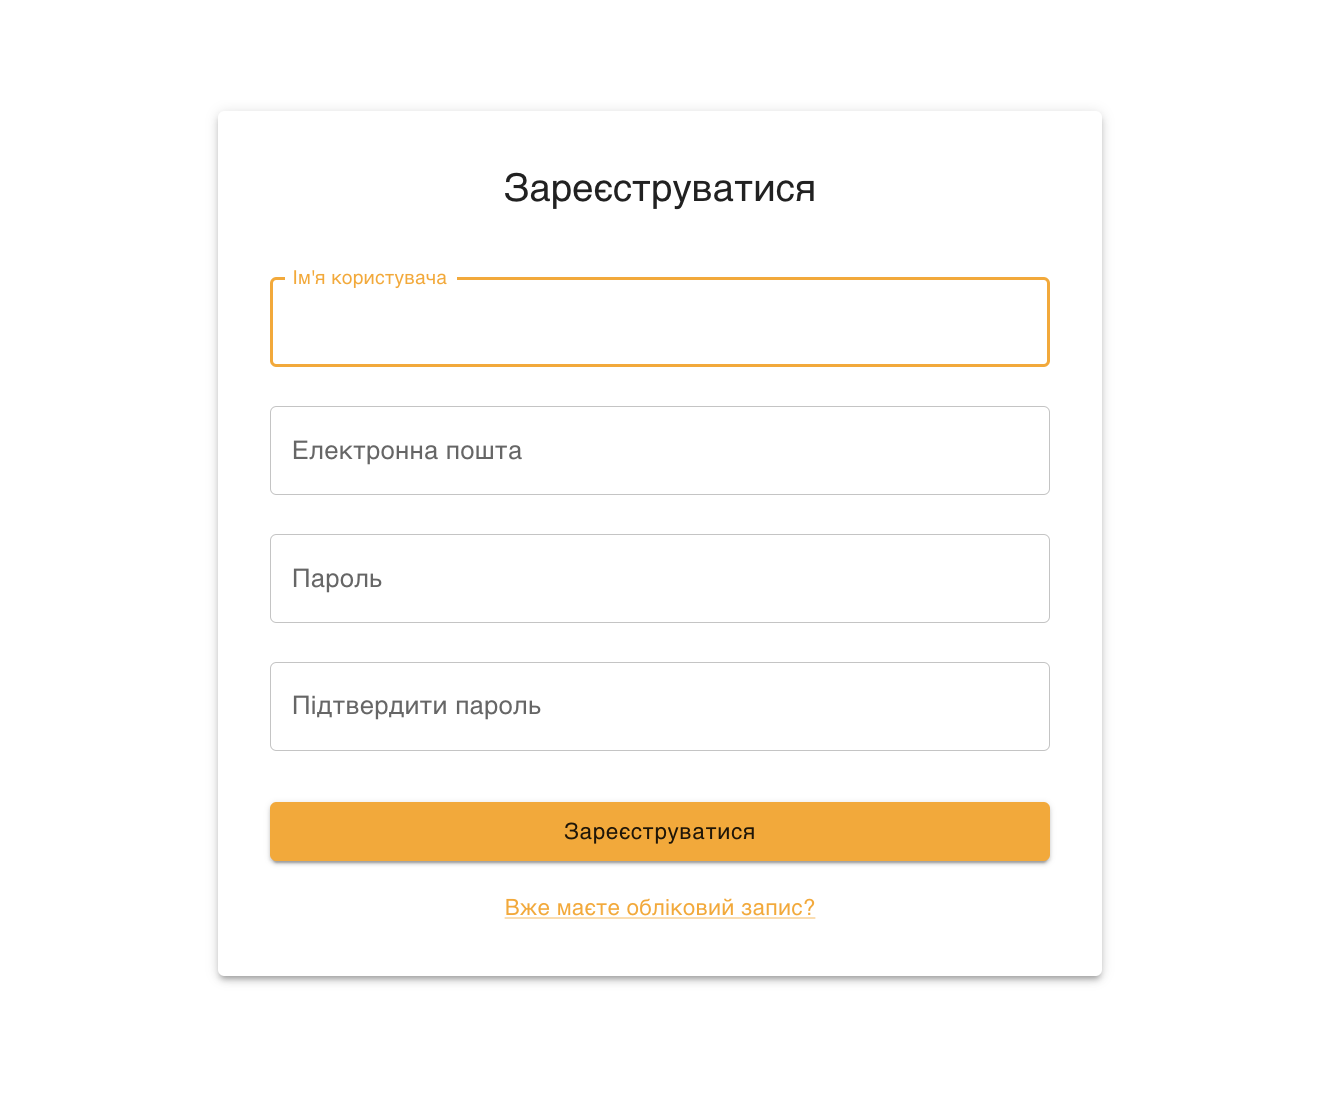
\includegraphics[width=0.6\textwidth]{practice_report/images/registration_form.png}
    \caption{Інтерфейс форми реєстрації нового користувача}
    \label{fig:registration_form}
\end{figure}

Детальна послідовність кроків, що включає як початкову реєстрацію, так і наступний етап верифікації електронної пошти через отриманий лист, ілюструється на діаграмі послідовності на рисунку \ref{fig:local_registration_flow}.

\begin{figure}[htbp]
    \centering
    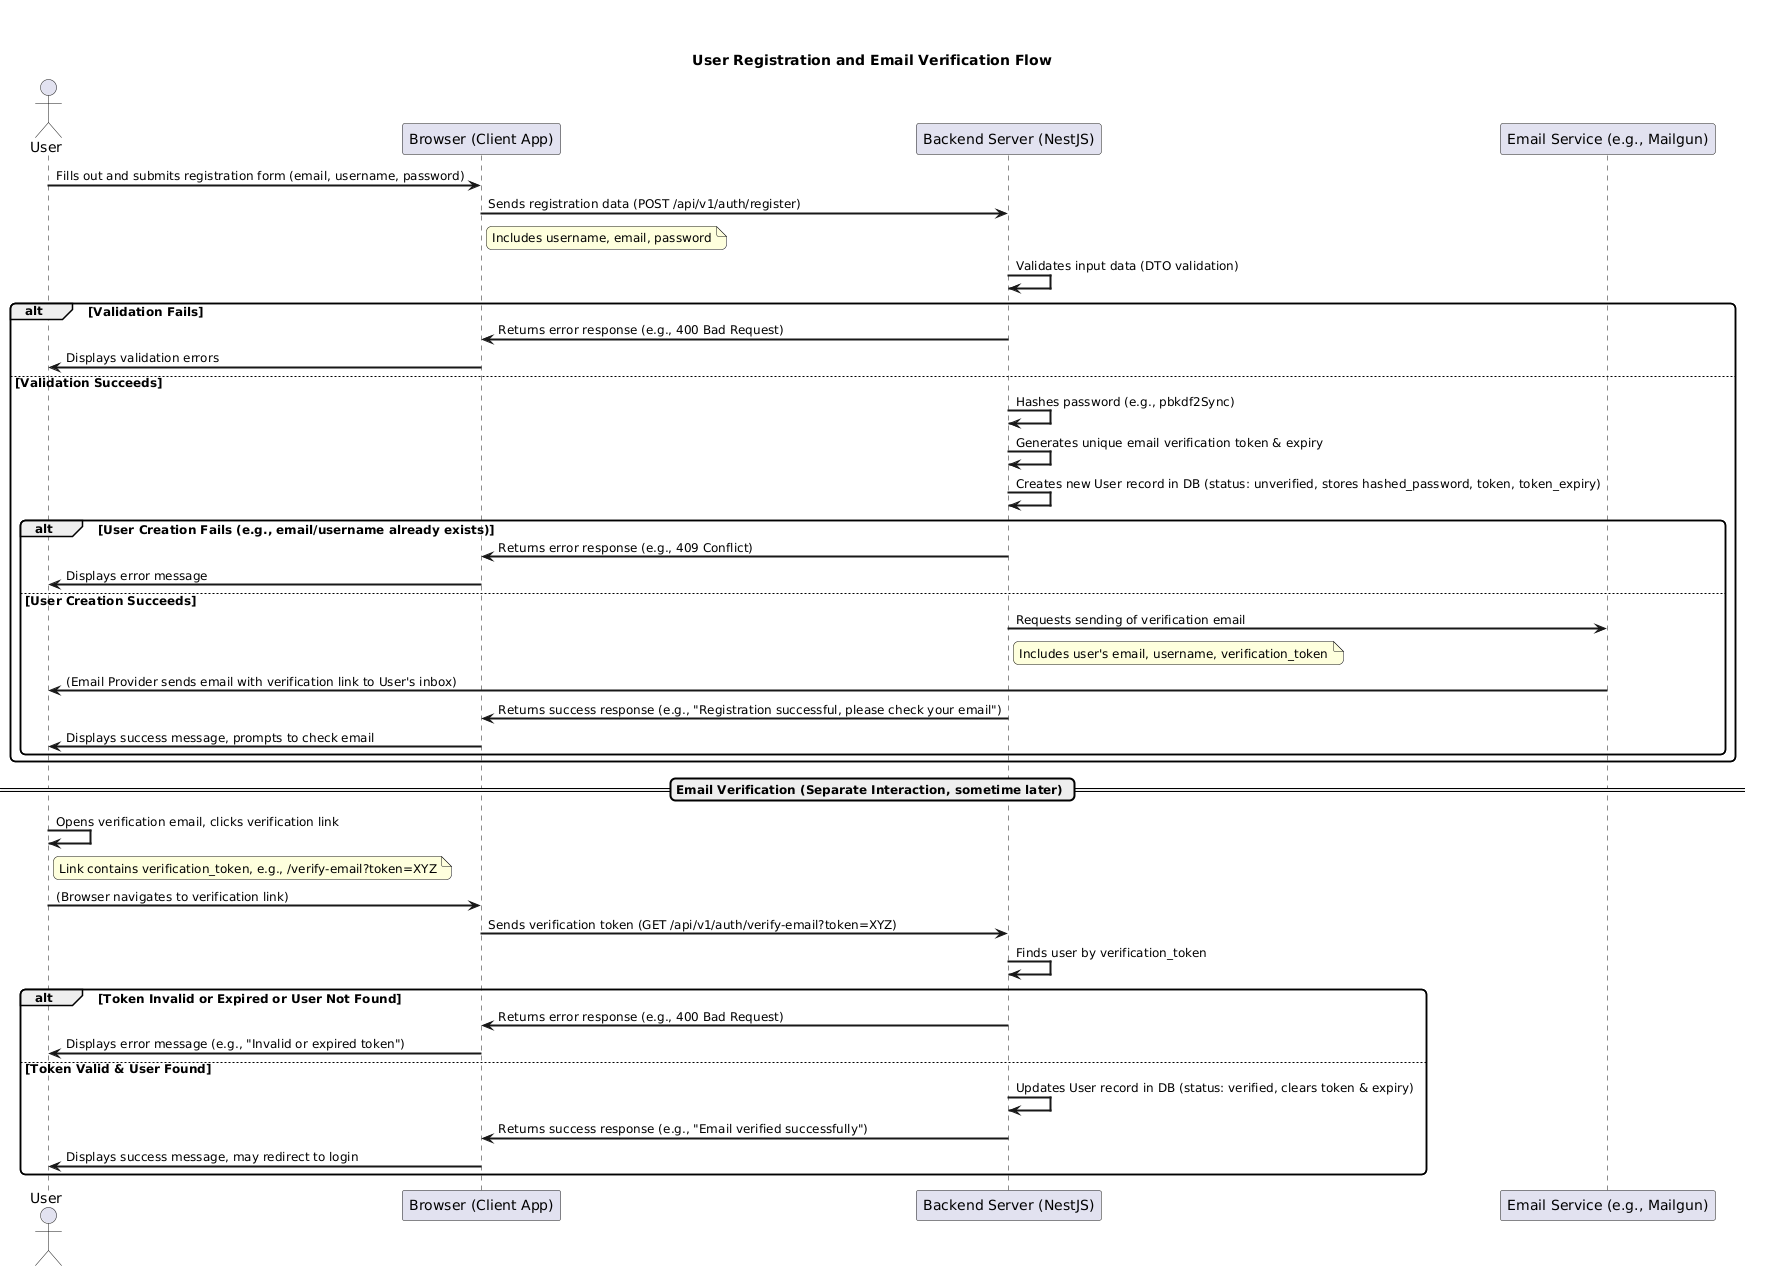
\includegraphics[width=\textwidth]{practice_report/images/local_registration_flow.png}
    \caption{Діаграма послідовності для реєстрації користувача та верифікації email}
    \label{fig:local_registration_flow}
\end{figure}

Центральним елементом процесу входу користувача є сторінка автентифікації, зображена на рисунку \ref{fig:login_page}. Інтерфейс надає поля для введення електронної пошти та пароля, кнопку для надсилання форми, а також посилання для переходу на сторінку реєстрації та кнопку для автентифікації через обліковий запис Google (використовуючи протокол OAuth 2.0). Після успішного введення облікових даних (або успішної автентифікації через Google) та їх перевірки на серверній стороні, користувач отримує доступ до захищених ресурсів платформи. Детальніше взаємодія між компонентами системи під час автентифікації, зокрема через Google, показана на діаграмі послідовності на рисунку \ref{fig:google_oauth_flow}.

\begin{figure}[htbp]
    \centering
    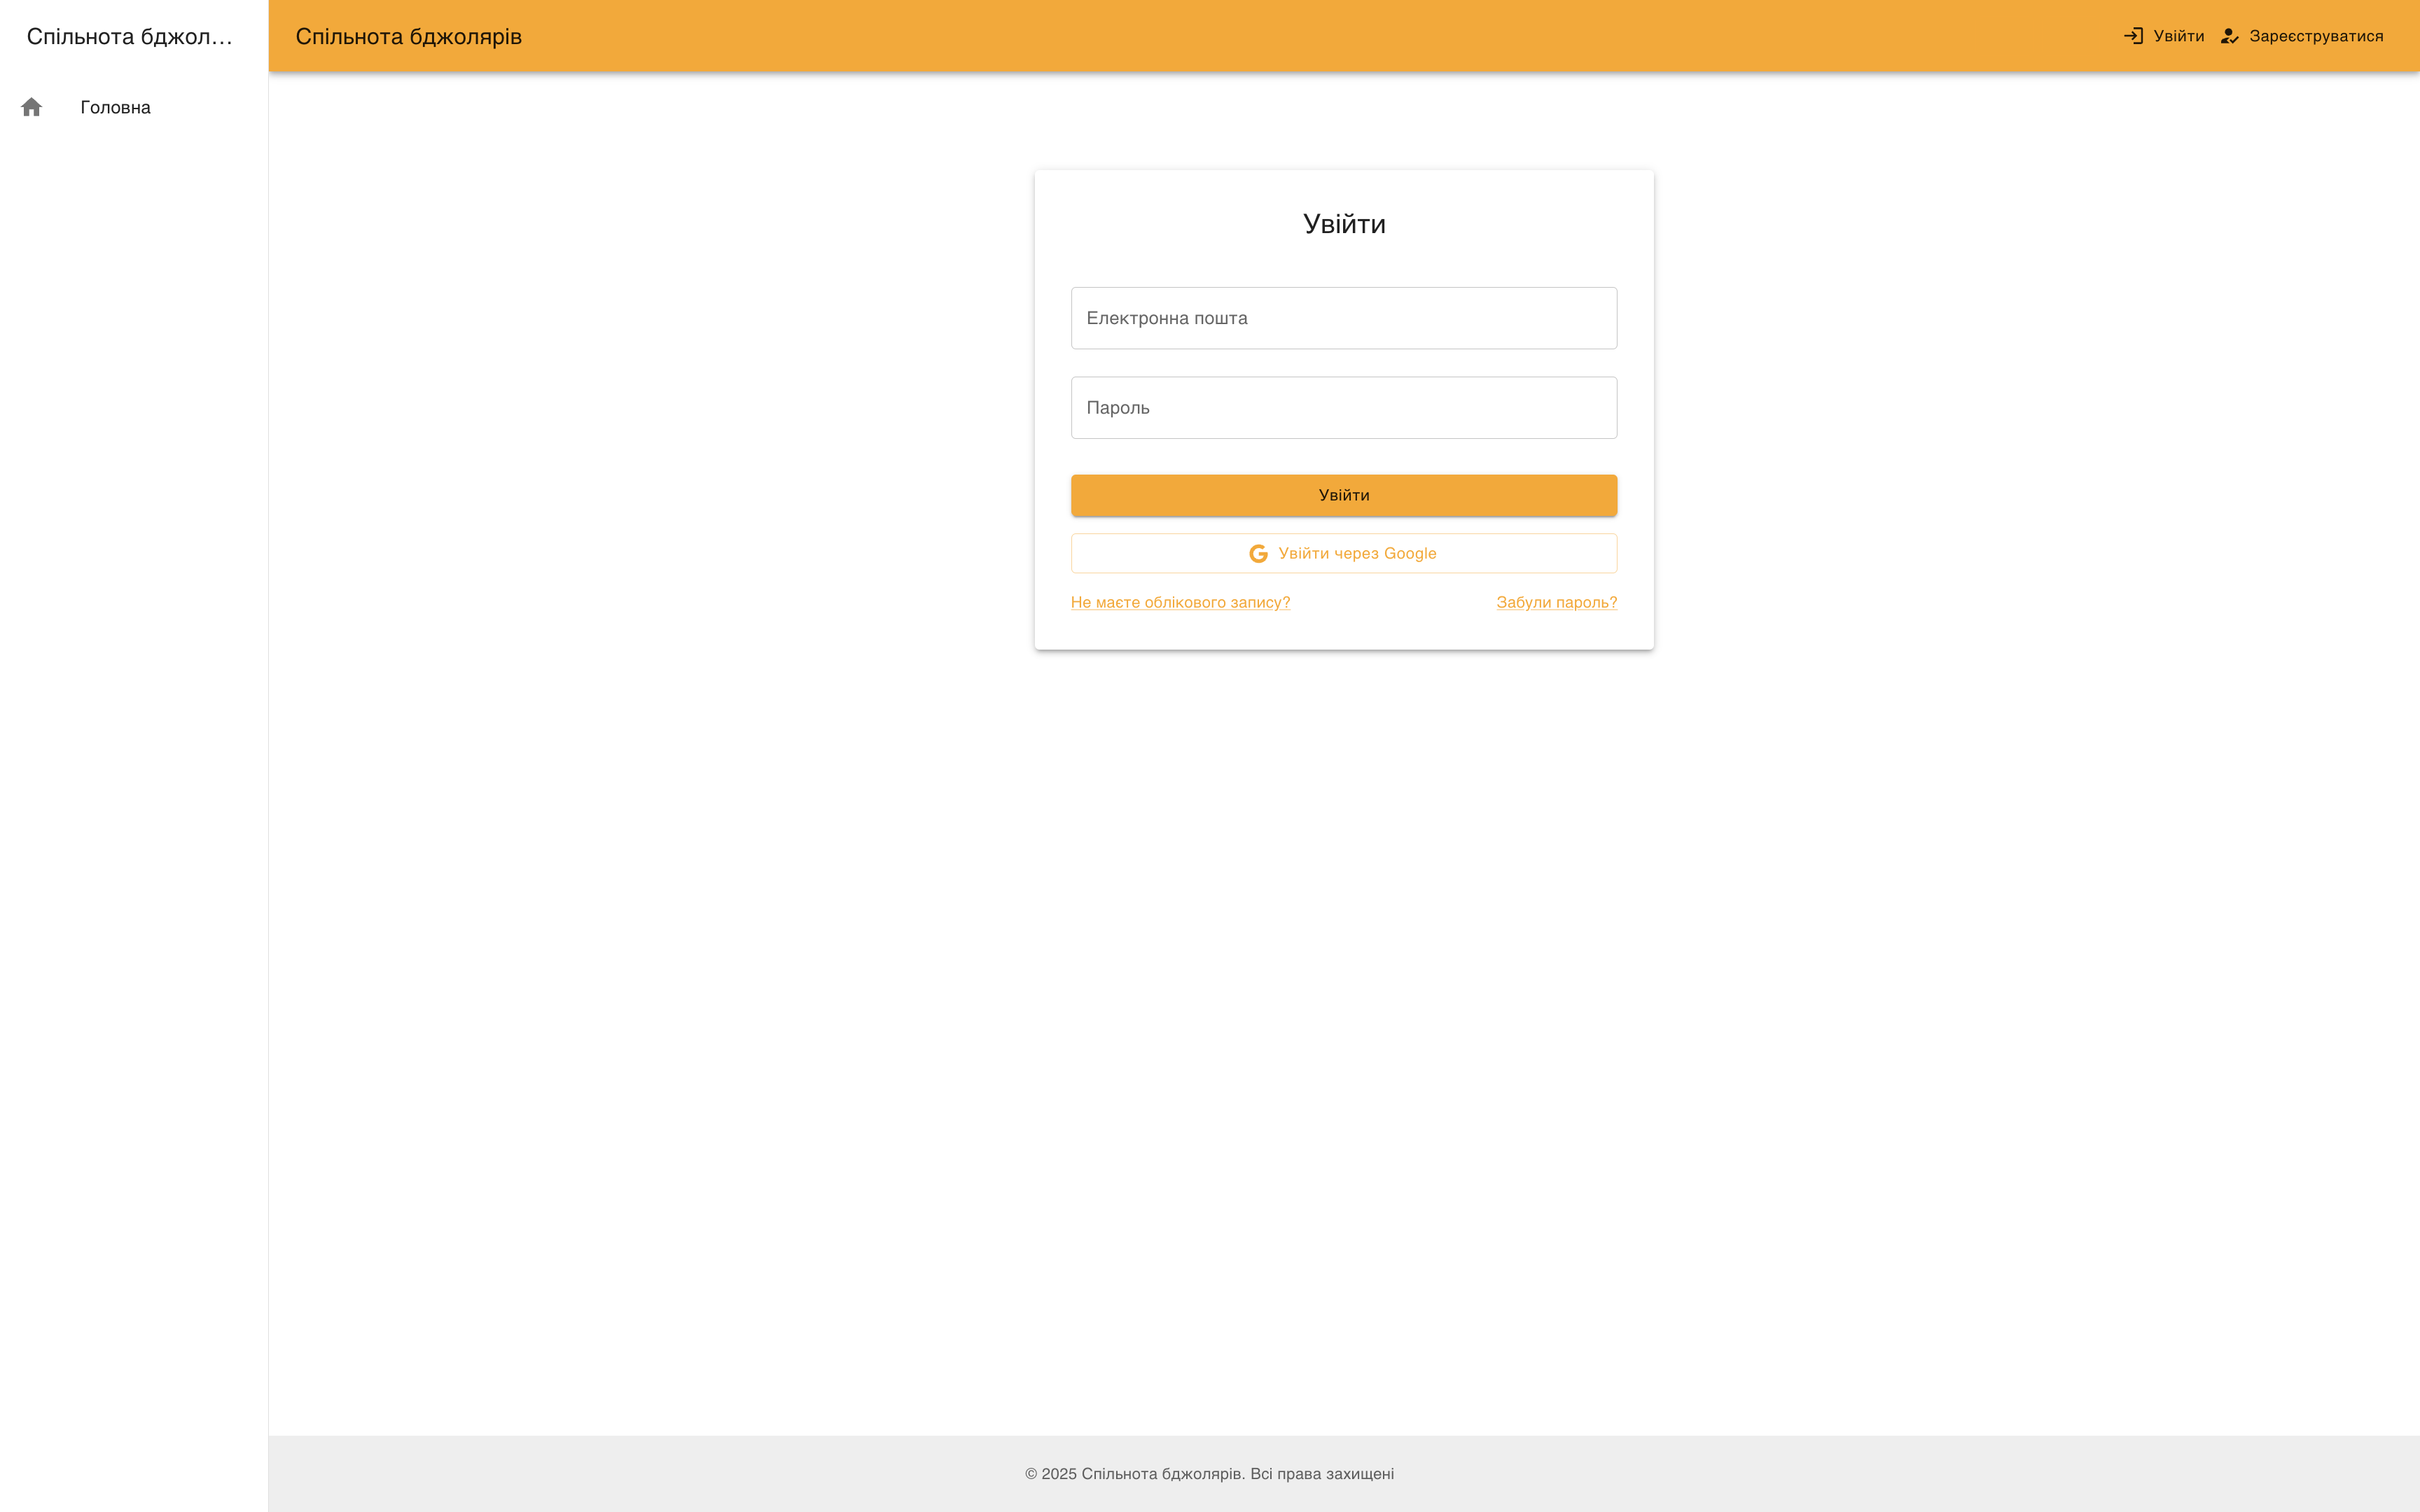
\includegraphics[width=0.8\textwidth]{practice_report/images/login_page.png}
    \caption{Інтерфейс сторінки входу до системи}
    \label{fig:login_page}
\end{figure}

Послідовність кроків, що виконуються під час автентифікації користувача за допомогою сервісу Google OAuth 2.0, включаючи взаємодію між клієнтом, серверною частиною платформи та сервером автентифікації Google, детально ілюстрована на рисунку \ref{fig:google_oauth_flow}.

\begin{figure}[htbp]
    \centering
    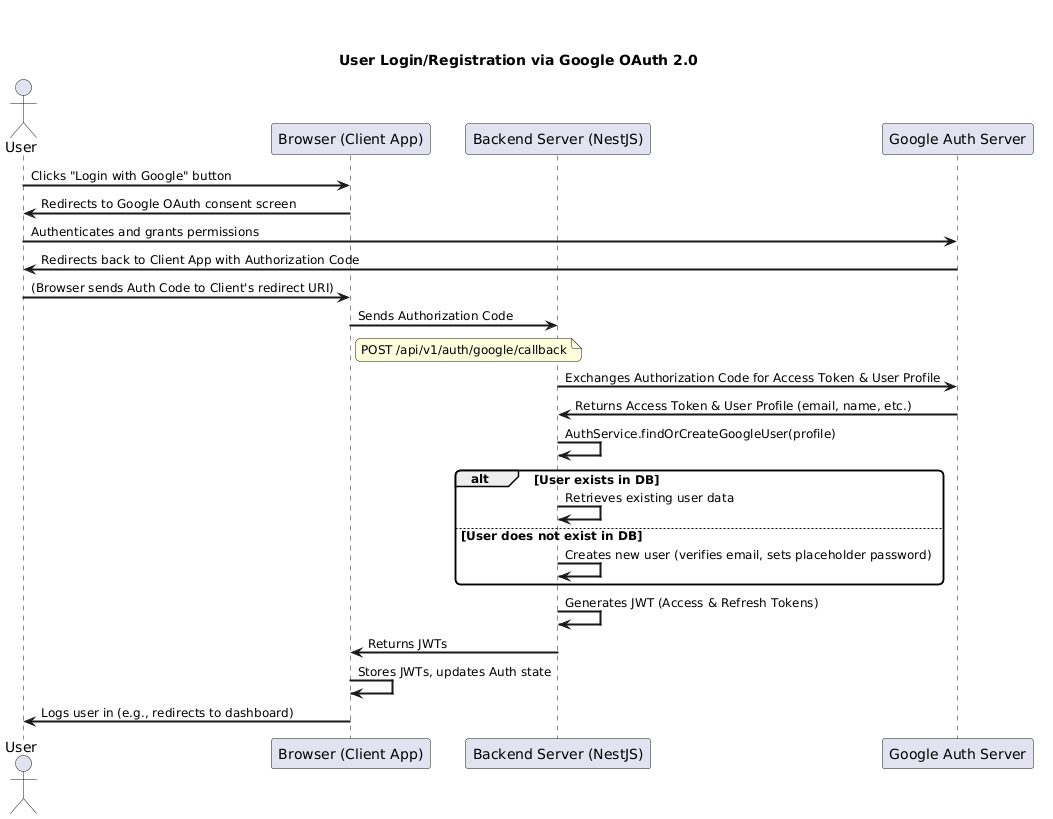
\includegraphics[width=\textwidth]{practice_report/images/google_oauth_flow.png}
    \caption{Послідовність дій при автентифікації через Google OAuth 2.0}
    \label{fig:google_oauth_flow}
\end{figure}

\subsection{Форум}
Модуль форуму дозволяє користувачам створювати теми для обговорення, залишати повідомлення та коментарі, а також висловлювати свою думку за допомогою лайків. Дані зберігаються в колекції \texttt{forumposts}. Фронтенд реалізований з використанням компонентів для списку постів, окремого поста та форми створення нового поста. Взаємодія з бекендом відбувається через відповідні API ендпоінти, реалізовані в \texttt{ForumController} та \texttt{ForumService}.

\subsection{База знань}
Модуль бази знань (на даний момент з демонстраційними даними на клієнті) передбачає зберігання та відображення статей, посібників та інших корисних матеріалів для бджолярів. Планується розширення функціоналу для управління контентом через адміністративну панель та реалізація повноцінного API для роботи з ресурсами бази знань.

\subsection{Інтеграція інтерактивної карти}
Одним з ключових функціональних блоків є інтерактивна карта, реалізована за допомогою Leaflet та React-Leaflet на фронтенді та GeoJSON з індексами \texttt{2dsphere} на бекенді (MongoDB). Компонент \texttt{MapPage.tsx} є центральним для цієї функціональності.

\subsubsection{Управління вуликами (Hives)}
Користувачі платформи мають можливість візуалізувати та управляти своїми вуликами безпосередньо на інтерактивній карті. Загальний вигляд розміщення вуликів на карті, включаючи їх маркери та спливаючі вікна з детальною інформацією, представлено на рисунку \ref{fig:map_hives_demo}.

\begin{figure}[htbp]
    \centering
    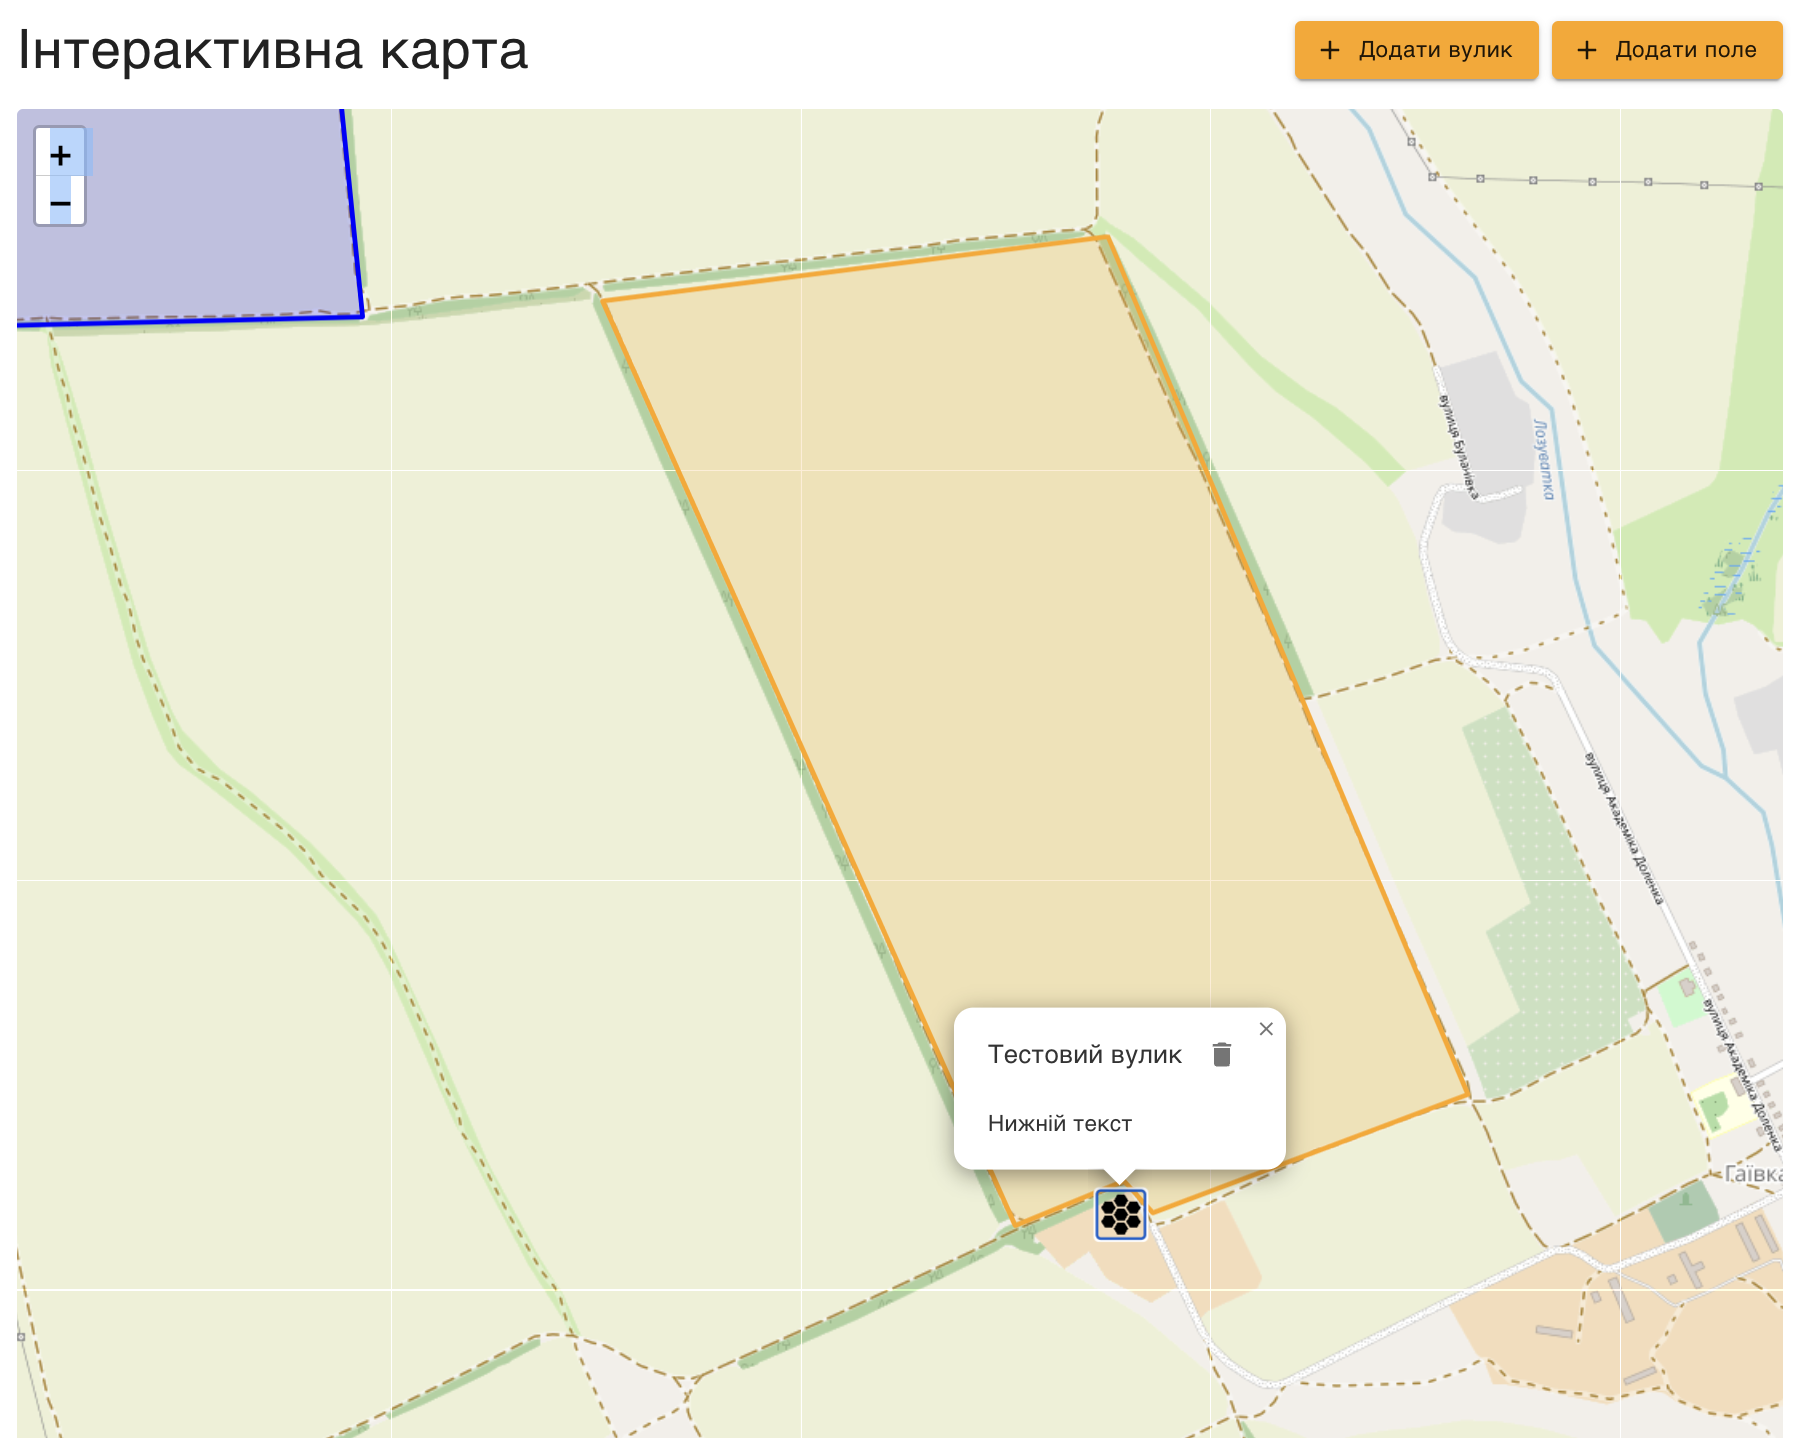
\includegraphics[width=0.8\textwidth]{practice_report/images/map_hives_demo.png}
    \caption{Демонстрація відображення вуликів на інтерактивній карті}
    \label{fig:map_hives_demo}
\end{figure}

\begin{itemize}
    \item \textbf{Додавання вуликів:} Користувачі можуть додавати на карту точкові маркери для позначення вуликів. Через діалогове вікно \texttt{AddHiveDialog.tsx} вказуються назва та нотатки. Геолокація визначається кліком на карті. Дані надсилаються на бекенд за допомогою RTK Query мутації \texttt{useAddHiveMutation}.
    
    \item \textbf{Відображення вуликів з кастомними іконками:} 
    Стандартні маркери бібліотеки Leaflet є досить загальними. Для покращення візуального сприйняття та тематичної відповідності було реалізовано відображення вуликів на карті за допомогою кастомних іконок. В якості візуального образу було обрано іконку \texttt{HiveIcon} з бібліотеки Material-UI, що забезпечує стилістичну єдність з іншими елементами інтерфейсу платформи. 
    
    Оскільки Leaflet очікує HTML-рядок або DOM-елемент для кастомних маркерів через \texttt{L.divIcon}, а \texttt{HiveIcon} є React-компонентом, було застосовано наступне рішення. За допомогою функції \texttt{ReactDOMServer.renderToString()} з пакету \texttt{react-dom/server} (яка зазвичай використовується для серверного рендерингу) React-компонент іконки перетворюється на статичний HTML-рядок на стороні клієнта. Цей рядок потім передається у властивість \texttt{html} об'єкта конфігурації \texttt{L.divIcon}. 
    
    При створенні кастомної іконки також налаштовуються важливі параметри \texttt{L.divIcon}, такі як \texttt{className} (для можливості додаткової стилізації за допомогою каскадних таблиць стилів (Cascading Style Sheets, CSS)), \texttt{iconSize} (розмір іконки), \texttt{iconAnchor} (точка прив'язки іконки до географічних координат, щоб вістря іконки вказувало на точне місце), та \texttt{popupAnchor} (позиціонування спливаючого вікна відносно іконки). Сформований таким чином об'єкт \texttt{hiveLeafletIcon} потім передається у пропс \texttt{icon} компонента \texttt{<Marker>} з бібліотеки React-Leaflet. Такий підхід дозволив ефективно інтегрувати React-компоненти Material-UI в картографічний контекст Leaflet, забезпечуючи кращий користувацький досвід та візуальну привабливість карти.

    \item \textbf{Видалення вуликів:} Користувачі можуть видаляти свої вулики. У спливаючому вікні (Popup) маркера вулика розміщена кнопка видалення. Натискання на неї активує діалогове вікно для підтвердження дії. Після підтвердження, мутація \texttt{useDeleteHiveMutation} з RTK Query відправляє запит на бекенд для видалення відповідного запису з колекції \texttt{hives}.
    \item \textbf{Перегляд інформації:} У спливаючому вікні (Popup) кожного вулика відображається його назва та нотатки.
\end{itemize}

\subsubsection{Управління полями (Fields)}
Аналогічно до вуликів, користувачі можуть додавати, переглядати та управляти інформацією про сільськогосподарські поля. На рисунку \ref{fig:map_fields_demo} показано, як поля відображаються у вигляді полігонів, разом зі спливаючими вікнами, що містять ключову інформацію, таку як тип культури та дати обробок.

\begin{figure}[htbp]
    \centering
    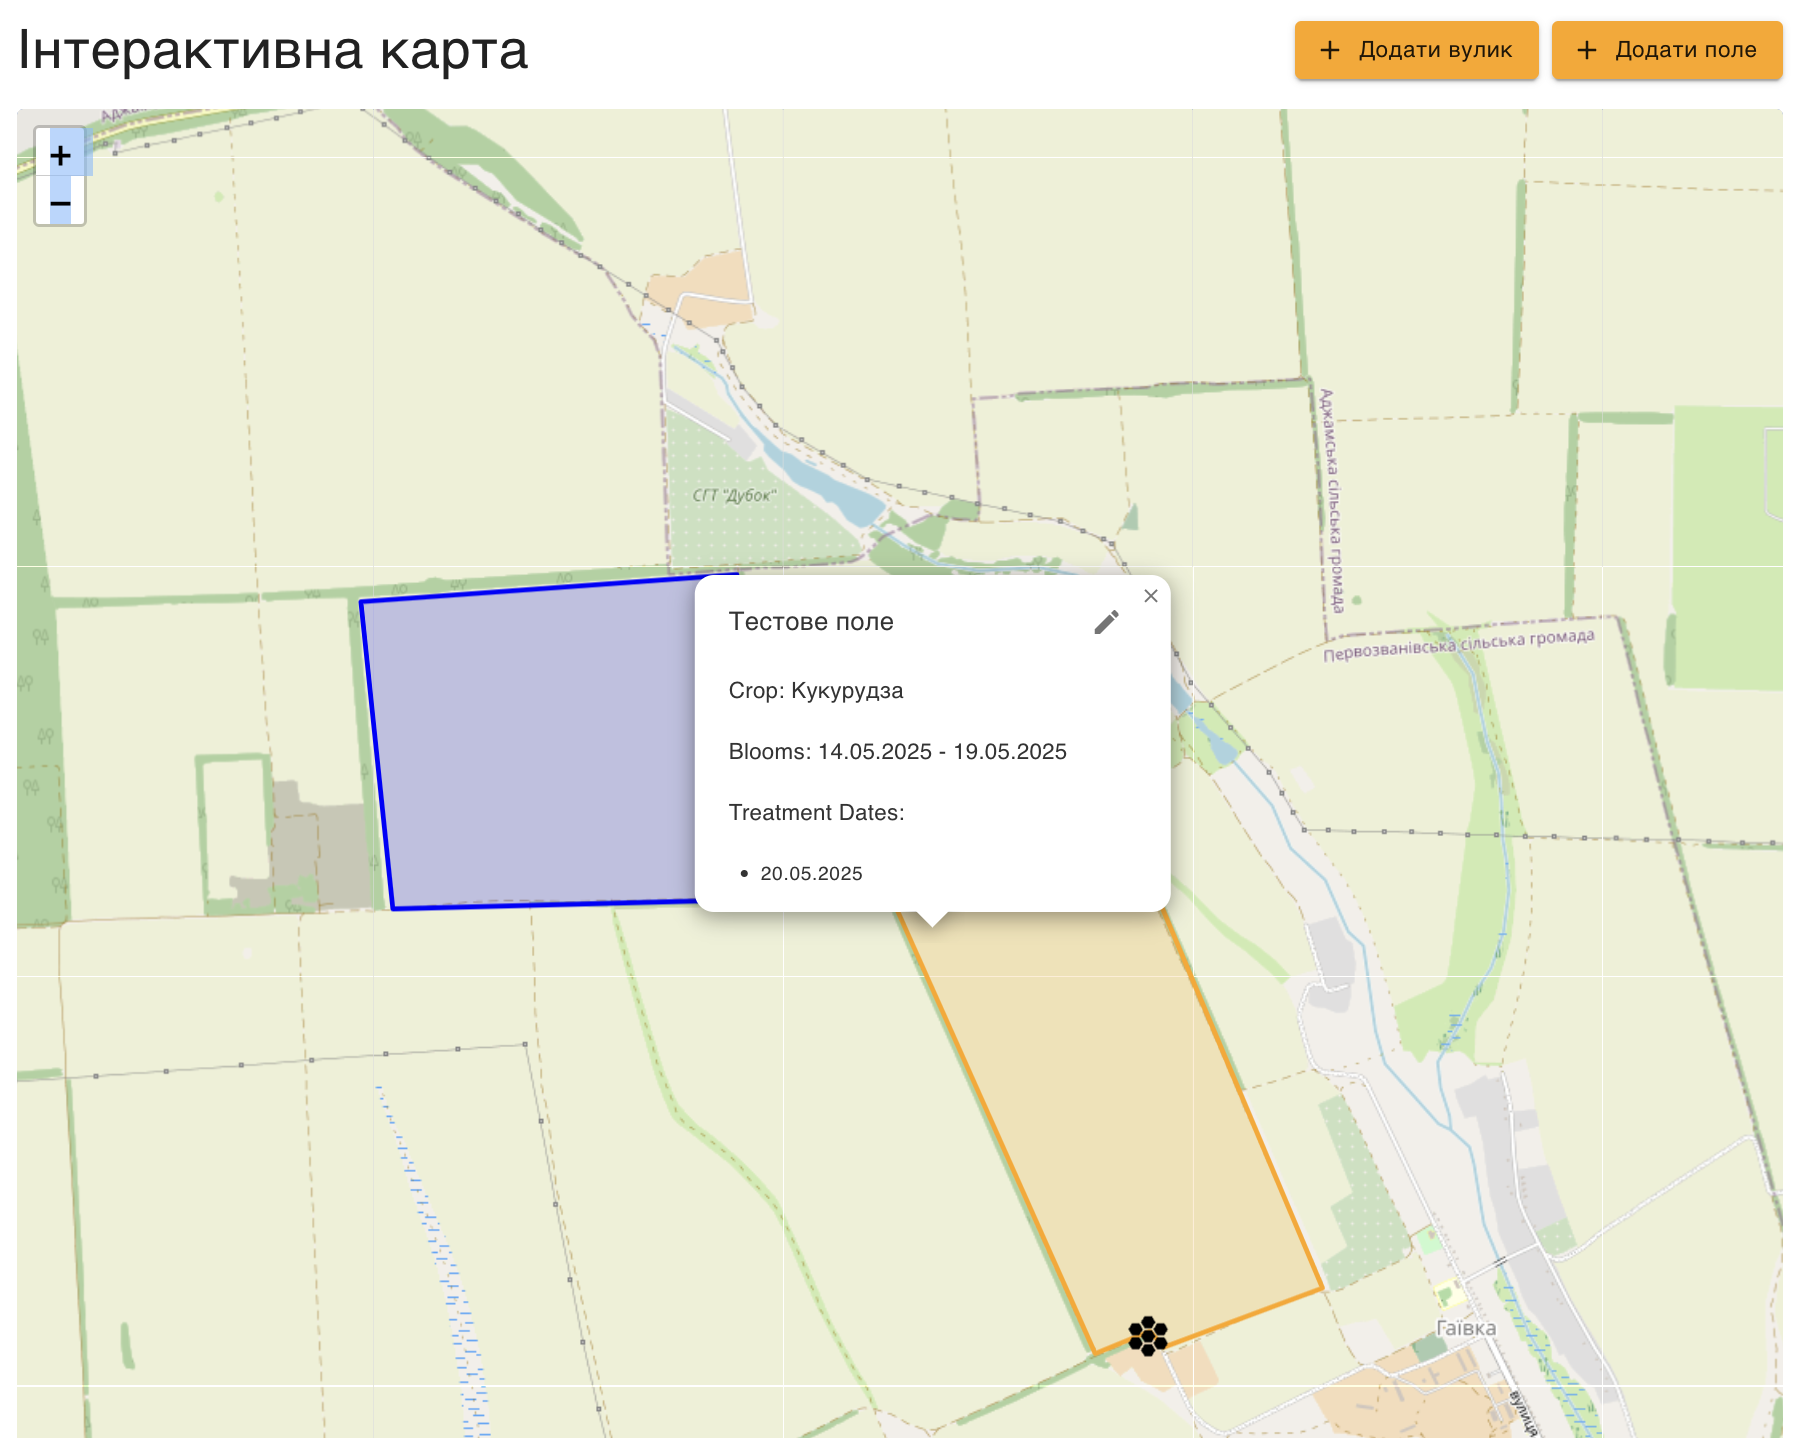
\includegraphics[width=0.8\textwidth]{practice_report/images/map_fields_demo.png}
    \caption{Демонстрація відображення полів на інтерактивній карті}
    \label{fig:map_fields_demo}
\end{figure}

\begin{itemize}
    \item \textbf{Додавання полів:} Користувачі можуть малювати полігони на карті для позначення полів. Діалогове вікно \texttt{AddFieldDialog.tsx} дозволяє вказати назву поля, тип культури, період цвітіння та список запланованих дат обробки. Геометрія полігону передається на бекенд у форматі GeoJSON. Використовується мутація \texttt{useAddFieldMutation}.
    
    \item \textbf{Відображення полів та візуалізація статусу обробки:} 
    Поля відображаються як полігони на карті за допомогою компонента \texttt{<Polygon>} з бібліотеки React-Leaflet. Ключовою особливістю є динамічна зміна кольору полігону для візуального інформування бджолярів про заплановані хімічні обробки полів, що можуть становити загрозу для бджіл. Ця логіка реалізована в компоненті \texttt{MapPage.tsx} у функції \texttt{getFieldTreatmentStatus}. 
    
    Функція приймає масив дат обробок для конкретного поля. Вона порівнює кожну дату обробки з поточною датою. Якщо обробка запланована на сьогодні, полю присвоюється червоний колір (високий ризик). Якщо обробка запланована протягом наступних семи днів (визначено константою \texttt{TREATMENT\_SOON\_DAYS}), полю присвоюється помаранчевий колір (середній ризик). В інших випадках використовується стандартний синій колір. Перевірка на "сьогодні" здійснюється за допомогою допоміжної функції \texttt{isSameDay}, яка порівнює рік, місяць та день двох дат. Результатом роботи \texttt{getFieldTreatmentStatus} є об'єкт, що містить властивість \texttt{color}, значення якої динамічно передається в атрибут \texttt{pathOptions} компонента \texttt{<Polygon>}. Для оптимізації та уникнення зайвих перерахунків при кожному рендері компонента, функція \texttt{getFieldTreatmentStatus} обгорнута в React хук \texttt{useMemo} (хоча в поточній реалізації без залежностей вона створюється один раз). Це забезпечує користувачам наочне та оперативне сповіщення про потенційні загрози.

    \item \textbf{Редагування метаданих полів:} 
    Для модифікації атрибутів існуючих полів було розроблено спеціалізований діалоговий компонент \texttt{EditFieldDialog.tsx}. Активація цього діалогу відбувається при натисканні користувачем кнопки редагування у спливаючому вікні (Popup) відповідного полігону поля на карті. Компонент отримує через пропси поточні дані поля (\texttt{initialData}), прапорець видимості (\texttt{open}), обробники закриття (\texttt{onClose}) та відправки форми (\texttt{onSubmit}), а також стан завантаження (\texttt{isLoading}) для індикації процесу взаємодії з API.
    
    Внутрішній стан форми (\texttt{formData}), що включає назву, тип культури, дати початку та кінця цвітіння, а також список дат обробки, управляється за допомогою хука \texttt{useState}. При відкритті діалогу або зміні \texttt{initialData}, хук \texttt{useEffect} відповідає за ініціалізацію стану форми даними обраного поля. Важливим аспектом є перетворення форматів дат: рядкові ISO-дати, отримані з бекенду, форматуються у вигляд \texttt{YYYY-MM-DD}, сумісний з HTML-елементами вводу типу \texttt{date}.
    
    Обробка змін у текстових полях форми реалізована через універсальний обробник \texttt{handleChange}. Для управління динамічним списком дат обробки передбачені окремі функції: \texttt{addTreatmentDate} для додавання нового поля вводу дати, \texttt{removeTreatmentDate} для видалення існуючого, та \texttt{handleTreatmentDateChange} для оновлення конкретної дати у списку. 
    
    При відправці форми функція \texttt{handleSubmit} виконує базову валідацію введених даних. Якщо валідація успішна, викликається переданий через пропси обробник \texttt{onSubmit} (визначений у \texttt{MapPage.tsx}). Цей обробник, у свою чергу, активує RTK Query мутацію \texttt{useUpdateFieldMutation}, передаючи ідентифікатор поля (\texttt{\_id}) та об'єкт \texttt{formData} з оновленими даними на сервер. Протягом виконання асинхронного запиту до API, пропс \texttt{isLoading} використовується для блокування елементів форми та відображення індикатора завантаження на кнопці збереження, забезпечуючи користувачеві зворотний зв'язок.

    \item \textbf{Перегляд інформації:} У спливаючому вікні (Popup) кожного поля відображається його назва, тип культури, період цвітіння та список дат обробки.
\end{itemize}

Бекенд надає відповідні CRUD (Create, Read, Update, Delete – Створити, Прочитати, Оновити, Видалити) API ендпоінти для управління вуликами та полями, забезпечуючи збереження, отримання, оновлення та видалення геопросторових об'єктів та їх метаданих (колекції \texttt{hives} та \texttt{fields} у MongoDB).

\subsection{Реалізація функціоналу адміністрування користувачів}
\label{subsec:admin_user_management}
Для забезпечення можливостей управління користувачами платформи було розроблено адміністративний функціонал, доступний лише користувачам з роллю адміністратора. Цей функціонал включає перегляд списку всіх користувачів та можливість зміни їх адміністративного статусу.

\subsubsection{Захист адміністративних маршрутів}
На серверній стороні доступ до адміністративних ендпоінтів контролюється за допомогою спеціалізованого NestJS Guard – \texttt{AdminGuard} (файл \texttt{server/src/auth/guards/admin.guard.ts}). Цей guard активується після успішної автентифікації користувача через \texttt{JwtAuthGuard}. \texttt{AdminGuard} перевіряє наявність поля \texttt{isAdmin} зі значенням \texttt{true} в об'єкті користувача, що додається до запиту \texttt{JwtAuthGuard}. Якщо користувач не є адміністратором, guard генерує виняток \texttt{ForbiddenException}, блокуючи доступ.

\subsubsection{Сервісні методи та контролери для управління користувачами}
У сервісі \texttt{UsersService} (\texttt{server/src/users/users.service.ts}) було додано два ключових методи для адміністративних потреб:
\begin{itemize}
    \item \texttt{findAllAdmin()}: Повертає повний список всіх документів користувачів з бази даних. На відміну від потенційних публічних методів отримання користувачів, цей метод призначений для надання адміністратору повного огляду.
    \item \texttt{updateUserAdminStatus(userIdToUpdate: string, isAdmin: boolean)}: Оновлює поле \texttt{isAdmin} для вказаного користувача. Метод знаходить користувача за \texttt{userIdToUpdate} та встановлює нове значення для його адміністративного статусу, повертаючи оновлений документ користувача.
\end{itemize}
Відповідні ендпоінти були додані до \texttt{UsersController} (\texttt{server/src/users/users.controller.ts}):
\begin{itemize}
    \item \texttt{GET /users/admin/all}: Викликає \texttt{usersService.findAllAdmin()} та захищений \texttt{JwtAuthGuard} і \texttt{AdminGuard}.
    \item \texttt{PATCH /users/admin/:userId/set-admin-status}: Приймає \texttt{userId} як параметр маршруту та тіло запиту типу \texttt{SetUserAdminStatusDto} (що містить поле \texttt{isAdmin: boolean}). Викликає \texttt{usersService.updateUserAdminStatus()} та також захищений обома guards.
\end{itemize}
Для валідації тіла запиту при зміні статусу адміністратора використовується DTO \texttt{SetUserAdminStatusDto} з відповідними декораторами \texttt{class-validator}.

\subsubsection{Клієнтська реалізація панелі адміністратора}
На клієнтській стороні було створено сторінку \texttt{AdminPage.tsx} (розташовану в \texttt{client/src/pages/}), яка слугує інтерфейсом для управління користувачами. Доступ до цієї сторінки контролюється на рівні компонента: перевіряється, чи поточний автентифікований користувач (отриманий за допомогою хука \texttt{useAuth} з \texttt{AuthContext}) має прапорець \texttt{isAdmin}, встановлений в \texttt{true}. Якщо користувач не є адміністратором, або дані про користувача ще завантажуються, відображається відповідне повідомлення про відмову в доступі або індикатор завантаження.

Для отримання списку всіх користувачів сторінка використовує RTK Query хук \texttt{useGetAllUsersAdminQuery} з \texttt{usersApi.ts}. Запит пропускається (опція \texttt{skip}), якщо поточний користувач не визначений як адміністратор. Отриманий список користувачів відображається за допомогою компонентів Material-UI \texttt{<List>}, \texttt{<ListItem>} та \texttt{<ListItemText>}, показуючи ім'я користувача, його email та ID. Поточний залогінений адміністратор візуально виділяється у списку.

Зміна адміністративного статусу користувача реалізована за допомогою компонента \texttt{<Switch>} (Material-UI) для кожного користувача у списку. Обробник \texttt{handleAdminStatusChange} викликається при зміні стану перемикача. Цей обробник ініціює RTK Query мутацію \texttt{useUpdateUserAdminStatusMutation}, передаючи ID користувача та нове значення статусу \texttt{isAdmin}. Для запобігання випадковій зміні власних прав, перемикач для поточного адміністратора деактивується. Після успішного виконання мутації (оновлення даних на сервері), викликається функція \texttt{refetch} (надана хуком \texttt{useGetAllUsersAdminQuery}) для оновлення списку користувачів на сторінці, що забезпечує актуальність відображених даних. Стани завантаження під час отримання списку (\texttt{isLoadingUsers}) та оновлення статусу (\texttt{isUpdatingStatus}) використовуються для відображення індикатора \texttt{<CircularProgress>}, надаючи користувачеві зворотний зв'язок про хід операцій. Текстові елементи на сторінці інтернаціоналізовані за допомогою хука \texttt{useTranslation} з \texttt{react-i18next}.

\subsection{Налаштування доставки транзакційних електронних листів}
\label{subsec:email_delivery}

Для забезпечення надійної та безпечної доставки транзакційних електронних листів (наприклад, для верифікації email), веб-платформа для комунікації та обміну знаннями в спільноті бджолярів \textit{Beekeepers Community Platform} інтегрується з сервісом Mailgun. Правильне налаштування системи доменних імен (Domain Name System, DNS) є критично важливим для доставки та відповідності сучасним галузевим стандартам, особливо тим, що висуваються великими провайдерами, такими як Google та Yahoo.

\subsubsection{Автентифікація домену}

Для автентифікації вихідних електронних листів до DNS-конфігурації домену проекту були додані наступні записи:

\begin{itemize}
    \item \textbf{SPF (Sender Policy Framework):} TXT-запис, що вказує, які поштові сервери мають право надсилати електронні листи від імені домену. Це допомагає запобігти несанкціонованим відправникам (спуфінгу).
    \item \textbf{DKIM (DomainKeys Identified Mail):} TXT-запис, що містить публічний криптографічний ключ. Вихідні листи підписуються приватним ключем Mailgun, а одержувачі можуть перевірити підпис за допомогою публічного ключа в DNS, забезпечуючи цілісність та автентичність повідомлення.
    \item \textbf{DMARC (Domain-based Message Authentication, Reporting, and Conformance):} TXT-запис, який інструктує приймаючі поштові сервери, як обробляти листи, що не пройшли перевірки SPF або DKIM.
        \begin{itemize}
            \item \textbf{Опції політики:}
                \begin{itemize}
                    \item \texttt{p=none}: Тільки моніторинг, без примусових дій.
                    \item \texttt{p=quarantine}: Відправляти листи, що не пройшли перевірку, до папки "Спам".
                    \item \texttt{p=reject}: Повністю блокувати листи, що не пройшли перевірку.
                \end{itemize}
            \item \textbf{Сучасна практика:} Через нові вимоги Google та Yahoo (з 2024 року), політика DMARC повинна бути встановлена щонайменше на \texttt{quarantine} або \texttt{reject} для використання у виробничому середовищі. Це захищає користувачів від фішингу та покращує доставку.
        \end{itemize}
\end{itemize}

\subsubsection{Поширення та верифікація DNS}

Після додавання необхідних записів, поширення змін у DNS може зайняти до 48 годин. Верифікація виконується за допомогою панелі керування Mailgun та сторонніх інструментів (наприклад, MXToolbox), щоб переконатися, що всі записи коректно опубліковані та доступні глобально.

\subsubsection{Безпека та відповідність стандартам}

\begin{itemize}
    \item \textbf{Відсутність жорстко закодованих облікових даних:} Усі API-ключі Mailgun та конфіденційні налаштування зберігаються у змінних середовища, а не в коді.
    \item \textbf{Постійний моніторинг:} Звіти DMARC надсилаються на визначену електронну адресу для моніторингу проблем автентифікації та потенційного зловживання.
    \item \textbf{Ескалація політики:} Проект спочатку використовує \texttt{p=none} для DMARC для моніторингу легітимного трафіку, а потім переходить до \texttt{quarantine} або \texttt{reject} для повної відповідності стандартам та захисту.
\end{itemize}

\subsubsection{Підсумкова таблиця DNS-записів}

\begin{table}[h!]
\centering
\begin{tabular}{|l|l|l|}
\hline
\textbf{Запис} & \textbf{Призначення} & \textbf{Приклад значення / Політика} \\
\hline
SPF    & Автентифікація відправника & \texttt{v=spf1 include:mailgun.org \~{}all} \\
DKIM   & Підпис повідомлення & (Публічний ключ, наданий Mailgun) \\
DMARC  & Політика та звіти & \texttt{v=DMARC1; p=quarantine; rua=mailto:admin@domain.com} \\
\hline
\end{tabular}
\caption{Приклади DNS-записів для автентифікації email.}
\label{tab:dns_records_email}
\end{table}

Така конфігурація гарантує, що всі вихідні електронні листи автентифіковані, знижуючи ризик спаму та фішингу та відповідаючи останнім вимогам основних поштових провайдерів. Вона також підтримує моніторинг та постійне вдосконалення безпеки електронної пошти.

\subsection{Реалізація інтелектуального FAQ-асистента}
\label{subsec:ai_faq_implementation}
Для надання користувачам швидких відповідей на поширені питання було реалізовано прототип інтелектуального FAQ-асистента, що використовує можливості великих мовних моделей (LLM), зокрема GPT-3.5-turbo від OpenAI \cite{openai_api}. Метою було дослідження потенціалу застосування LLM для покращення користувацького досвіду та оперативності надання інформації в рамках платформи.

\subsubsection{Серверна частина (Backend): Промпт-інжиніринг та взаємодія з OpenAI}
На бекенді, в модулі \texttt{FaqModule}, ключову роль відіграє \texttt{FaqService}. Цей сервіс відповідає за підготовку даних, конструювання промпту та взаємодію з API OpenAI.
\begin{itemize}
    \item \textbf{DTO запиту та Контролер:} Як і в інших модулях, використовується DTO \texttt{AskFaqDto} для валідації вхідного питання від користувача, яке надходить на ендпоінт \texttt{POST /api/v1/faq/ask}, оброблюваний \texttt{FaqController}.
    
    \item \textbf{Управління API-ключем:} API-ключ для доступу до OpenAI завантажується з конфігураційних файлів (змінних середовища) через \texttt{ConfigService}. Реалізовано перевірку наявності ключа при ініціалізації сервісу; у разі його відсутності, функціонал FAQ стає недоступним, про що логується попередження та інформується користувач при спробі запиту.

    \item \textbf{Побудова промпту – ядро логіки сервісу:}
    Якість відповіді LLM значною мірою залежить від якості та структури наданого промпту. У поточній реалізації прототипу застосовано наступний підхід до промпт-інжинірингу в методі \texttt{answerQuestion}:
    \begin{enumerate}
        \item \textbf{Формування контексту з ЧаПи (FAQ):} На даному етапі використовується статичний масив \texttt{FAQ\_DATA}, що містить пари «питання-відповідь». Перед відправкою до LLM, цей масив перетворюється на текстовий блок, де кожне питання та відповідь чітко позначені (наприклад, Q1:/A1:, Q2:/A2:). Це допомагає моделі розрізняти окремі елементи ЧаПи. 
        \textit{Обмеження поточного підходу до контексту:} Основне обмеження полягає в тому, що весь обсяг \texttt{FAQ\_DATA} включається в кожен запит. Зі зростанням кількості ЧаПи, це призведе до перевищення ліміту токенів, який підтримує обрана модель (наприклад, gpt-3.5-turbo має ліміт близько 4096 токенів для промпту та відповіді разом). Це робить поточне рішення не масштабованим для великих баз знань і слугує обґрунтуванням для впровадження семантичного пошуку в майбутньому.
        
        \item \textbf{Розробка системного повідомлення (System Prompt):} Системне повідомлення є критично важливим для керування поведінкою LLM. Для даного асистента воно було сформульовано таким чином, щоб чітко визначити роль моделі, обмежити джерело її знань та задати стиль відповіді:
        \begin{quote}
        \textit{Ви є корисним асистентом для платформи "Beekeepers Community Platform". Ваше завдання - відповідати на питання користувачів, базуючись ВИКЛЮЧНО на наданому контексті з ЧаПи (Часто Задаваних Питань). Якщо відповіді немає в контексті, чітко вкажіть, що ви не можете надати відповідь на основі наявної інформації. Не вигадуйте відповіді. Будьте коротким та чітким. Відповідайте українською мовою.}
        \end{quote}
        Ключові елементи цього промпту – вимога базуватися \textbf{виключно} на наданому контексті та інструкція щодо поведінки у випадку відсутності інформації – спрямовані на мінімізацію «галюцинацій» моделі (генерування неправдивої або нерелевантної інформації) та забезпечення того, що користувачі отримують відповіді, що стосуються саме платформи.
        
        \item \textbf{Конструювання фінального запиту до моделі:} Питання користувача, попередньо підготовлений контекст ЧаПи та системне повідомлення об'єднуються в структурований запит (у форматі повідомлень для Chat Completions API OpenAI), який надсилається до моделі. Це забезпечує чітке розділення інструкцій, контекстуальних даних та запиту користувача.
    \end{enumerate}

    \item \textbf{Взаємодія з OpenAI API та параметризація:}
    Для взаємодії з API використовується офіційна бібліотека \texttt{openai} для Node.js. Було обрано модель \texttt{gpt-3.5-turbo} як збалансований варіант за співвідношенням можливостей та вартості. Ключові параметри запиту до API включають:
    \begin{itemize}
        \item \texttt{model}: Назва використовуваної моделі.
        \item \texttt{messages}: Масив об'єктів, що включає системне повідомлення та повідомлення користувача (з контекстом та питанням).
        \item \texttt{temperature}: Встановлено на низьке значення (наприклад, 0.2 з діапазону 0 до 2) для зменшення випадковості та отримання більш детермінованих, фактологічних відповідей, що є бажаним для FAQ-системи.
        \item \texttt{max\_tokens}: Обмежує максимальну довжину генерованої відповіді (наприклад, 150-250 токенів), що допомагає контролювати витрати та стислість відповіді.
    \end{itemize}
    
    \item \textbf{Обробка відповіді та помилок:} Отримана від OpenAI відповідь проходить базову обробку (наприклад, видалення зайвих пробілів) перед поверненням на клієнт. Реалізовано логування запитів та відповідей, а також обробку потенційних помилок під час виклику API, з поверненням відповідного повідомлення користувачу.

\end{itemize}
На момент підготовки тез, для контрольованого запуску та уникнення непередбачених витрат, \texttt{FaqModule} закоментовано в основному модулі серверного застосунку (\texttt{AppModule}), що робить ендпоінт \texttt{/api/v1/faq/ask} тимчасово недоступним.

\subsubsection{Клієнтська частина (Frontend)}
На фронтенді реалізовано компонент \texttt{FaqSection.tsx} (у \texttt{client/src/components/faq/}), який надає користувацький інтерфейс для взаємодії з FAQ-асистентом. 
\begin{itemize}
    \item \textbf{Інтерфейс користувача:} Компонент містить текстове поле (MUI \texttt{<TextField>}) для введення питання та кнопку (MUI \texttt{<Button>}) для відправки запиту. Відповідь від асистента відображається в окремому блоці.
    \item \textbf{Взаємодія з API:} Для надсилання запиту на бекенд та отримання відповіді створено окремий RTK Query API slice \texttt{faqApi.ts} (у \texttt{client/src/store/api/}). Він визначає мутацію \texttt{useAskFaqMutation}.
    \item \textbf{Управління станом:} Компонент \texttt{FaqSection} використовує хук \texttt{useState} для зберігання поточного питання та отриманої відповіді. Стан завантаження (\texttt{isLoading}) та можливі помилки (\texttt{error}), що повертаються хуком \texttt{useAskFaqMutation}, використовуються для відображення індикатора завантаження (MUI \texttt{<CircularProgress>}) та повідомлень про помилки.
    \item \textbf{Інтеграція:} Компонент \texttt{FaqSection} інтегровано на сторінку Бази Знань (\texttt{KnowledgeBase.tsx}), хоча його рендеринг може бути керований feature-прапорцем для поступового впровадження.
\end{itemize}

\section{Безпека системи}
\label{sec:security_considerations}
При розробці увага приділялася аспектам безпеки:
\begin{itemize}
    \item \textbf{Автентифікація та авторизація:} Використання JWT, захист маршрутів, OAuth 2.0.
    \item \textbf{Зберігання паролів:} Паролі користувачів хешуються на стороні сервера перед збереженням у базу даних (використано модуль \texttt{crypto} Node.js, зокрема \texttt{pbkdf2Sync}).
    \item \textbf{Валідація вхідних даних:} Усі дані, що надходять від клієнта на бекенд, валідуються за допомогою DTO та \texttt{class-validator}, що запобігає некоректним даним та потенційним атакам (наприклад, NoSQL ін'єкції на рівні структури даних).
    \item \textbf{Захист від XSS:} Використання React на фронтенді за замовчуванням екранує дані, що вставляються в DOM, що знижує ризик XSS-атак.
    \item \textbf{CORS:} Налаштовано політику Cross-Origin Resource Sharing для контролю доступу до API з боку фронтенду.
    \item \textbf{Використання HTTPS:} У продакшн-середовищі необхідно використовувати HTTPS для шифрування трафіку.
    \item \textbf{Управління секретами:} Чутливі дані (секрети JWT, ключі API для зовнішніх сервісів, рядок підключення до БД) зберігаються у змінних середовища та не включаються до системи контролю версій.
\end{itemize} 